\documentclass[12pt]{article}
\usepackage[a4paper]{geometry}
\usepackage{fullpage}
\usepackage[T1]{fontenc}
\usepackage[utf8]{inputenc}
\usepackage{graphicx}
\usepackage{mathpazo}
\pagenumbering{gobble}
\usepackage{siunitx}
\sisetup{output-decimal-marker = {,}}
\usepackage{amsmath}
\usepackage{esdiff}
\usepackage[spanish]{babel}
\newcommand{\laplace}[1]{\mathbf{#1}(\mathbf{s})}
\newcommand{\slp}{\mathbf{s}}

\begin{document}

\title{\textsc{Teoría de Circuitos III}\\Prueba BT2}

\date{30 de octubre de  2018\\\small{Los resultados se publicarán el día 31 de octubre.\\La revisión del examen se realizará en horario de tutoría los días 6, 7 y 8 de noviembre.}}

\maketitle

El interruptor del circuito de la figura ha permanecido abierto un tiempo elevado, y se cierra en $t = 0$. En estas condiciones debe realizar el siguiente itinerario:

\begin{enumerate}
\item (\textbf{0,5p.}) Determinar las condiciones iniciales de las variables $u_C(0^+)$, $i_L(0^+)$, $i_R(0^+)$.
\item (\textbf{0,5p.}) Determinar los valores en régimen permanente de las variables $u_C(\infty)$, $i_L(\infty)$, $i_R(\infty)$.
\item (\textbf{4p.}) Dibujar el circuito en el dominio de Laplace para $t > 0$, y resolverlo para obtener las expresiones analíticas de $\laplace{I_L}$, $\laplace{U_C}$, $\laplace{I_R}$.
\item (\textbf{1p.}) Comprobar mediante los teoremas de valor inicial y valor final que las expresiones anteriores se ajustan a los resultados de los apartados 1 y 2.

\item (\textbf{1p.}) A partir de las expresiones obtenidas en el apartado 3, indique de forma razonada el tipo de transitorio existente en el circuito.

\item (\textbf{3p.}) Expresión en el dominio del tiempo de la variable $i_R(t)$.
\end{enumerate}

\begin{minipage}{0.3\textwidth}
Datos:
\begin{align*}
  E_g &= \SI{4}{\volt}\\
  R_1&= \SI{2}{\ohm}\\
  L &= \SI{1}{\henry}\\
  C &= \SI{250}{\milli\farad}\\
  R_2 &= \SI{2}{\ohm}
\end{align*}
\end{minipage}
\begin{minipage}{0.7\textwidth}
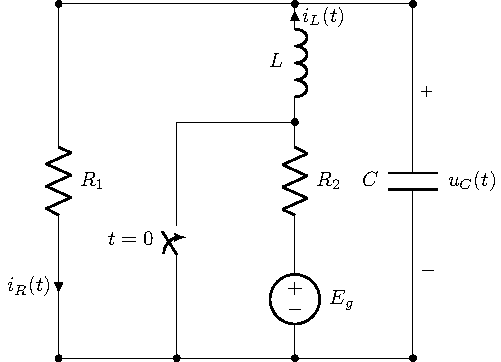
\includegraphics{figs/E2_circuito_v2.pdf}
\end{minipage}


\end{document}

% Local Variables:
% ispell-local-dictionary: "castellano"
% End:

